%\documentclass[handout]{beamer} %no pauses
\documentclass{beamer} %with pauses


\usetheme{copenhagen}
\usepackage{amsfonts}
\usepackage{mathtools}
\usepackage{graphicx}
\usepackage{amsmath}
\usepackage{url}

\newcommand{\bfrac}[2]{\frac{\displaystyle #1}{\displaystyle #2}}
\newcommand{\inner}[1]{\left\langle #1 \right\rangle}
\newcommand{\abs}[1]{\left\lvert #1 \right\rvert}
\newcommand{\norm}[1]{\left\lvert\left\lvert #1 \right\rvert\right\rvert}
\graphicspath{{./Images/}}

%Information to be included in the title page:
\title{MA 556 PRESENTATION}
\author{ANKAN MUKHERJEE}
\institute{IIT BOMBAY}
\date{\today}

\begin{document}

\frame{\titlepage}

\section{A Visual Argument for Sectional Curvature}

\begin{frame}
\frametitle{Sectional Curvature}
\begin{block}{Definition of Sectional Curvature}
Let $M$ be a Riemann manifold. Let $\sigma$ be a two dimensional subspace of $T_pM$ Let $(v,w)$ be a basis of $\sigma$. Then the scalar curvature is defined as
\begin{align}
\label{def}
K(v,w)=\bfrac{\inner{R(v,w)w,v)}}{\abs{v\wedge w}^2}
\end{align}
\end{block}
\pause
Note that the above definition of the sectional curvature is independent of the choice of basis $(v,w)$ and is thus a property of the plane $\sigma$ alone. This will be proven in the slides to come.
\end{frame}

\begin{frame}
\frametitle{Intuitive Version of Sectional Curvature}
Here we will intuitively see why the sectional curvature takes the form as given in \ref{def}. Note that the intuitive version presented in these slides is a culmination of various sources on the internet presenting several viewpoints on the topic.
\pause
I will be using geodesics as the starting point for the intuition behind curvature. Note that the definition of geodesic is a curve on a surface along which the distance between two points is the shortest. This can also be interpreted as the path that parallel transport of a vector along itself takes.
\pause
We will use a vector field of the tangent vectors on the family of geodesics, denoted by $V$ and the vector field orthogonal to it, denoted by $S$. Note that we can use the vectors in $S$ to estimate the distance between geodesics at a given point.
\end{frame}

\begin{frame}
\frametitle{Figure for Intuitive Version of Sectional Curvature}
\begin{figure}[!htb]
	\centering
   \begin{minipage}{0.8\textwidth}
     \centering
     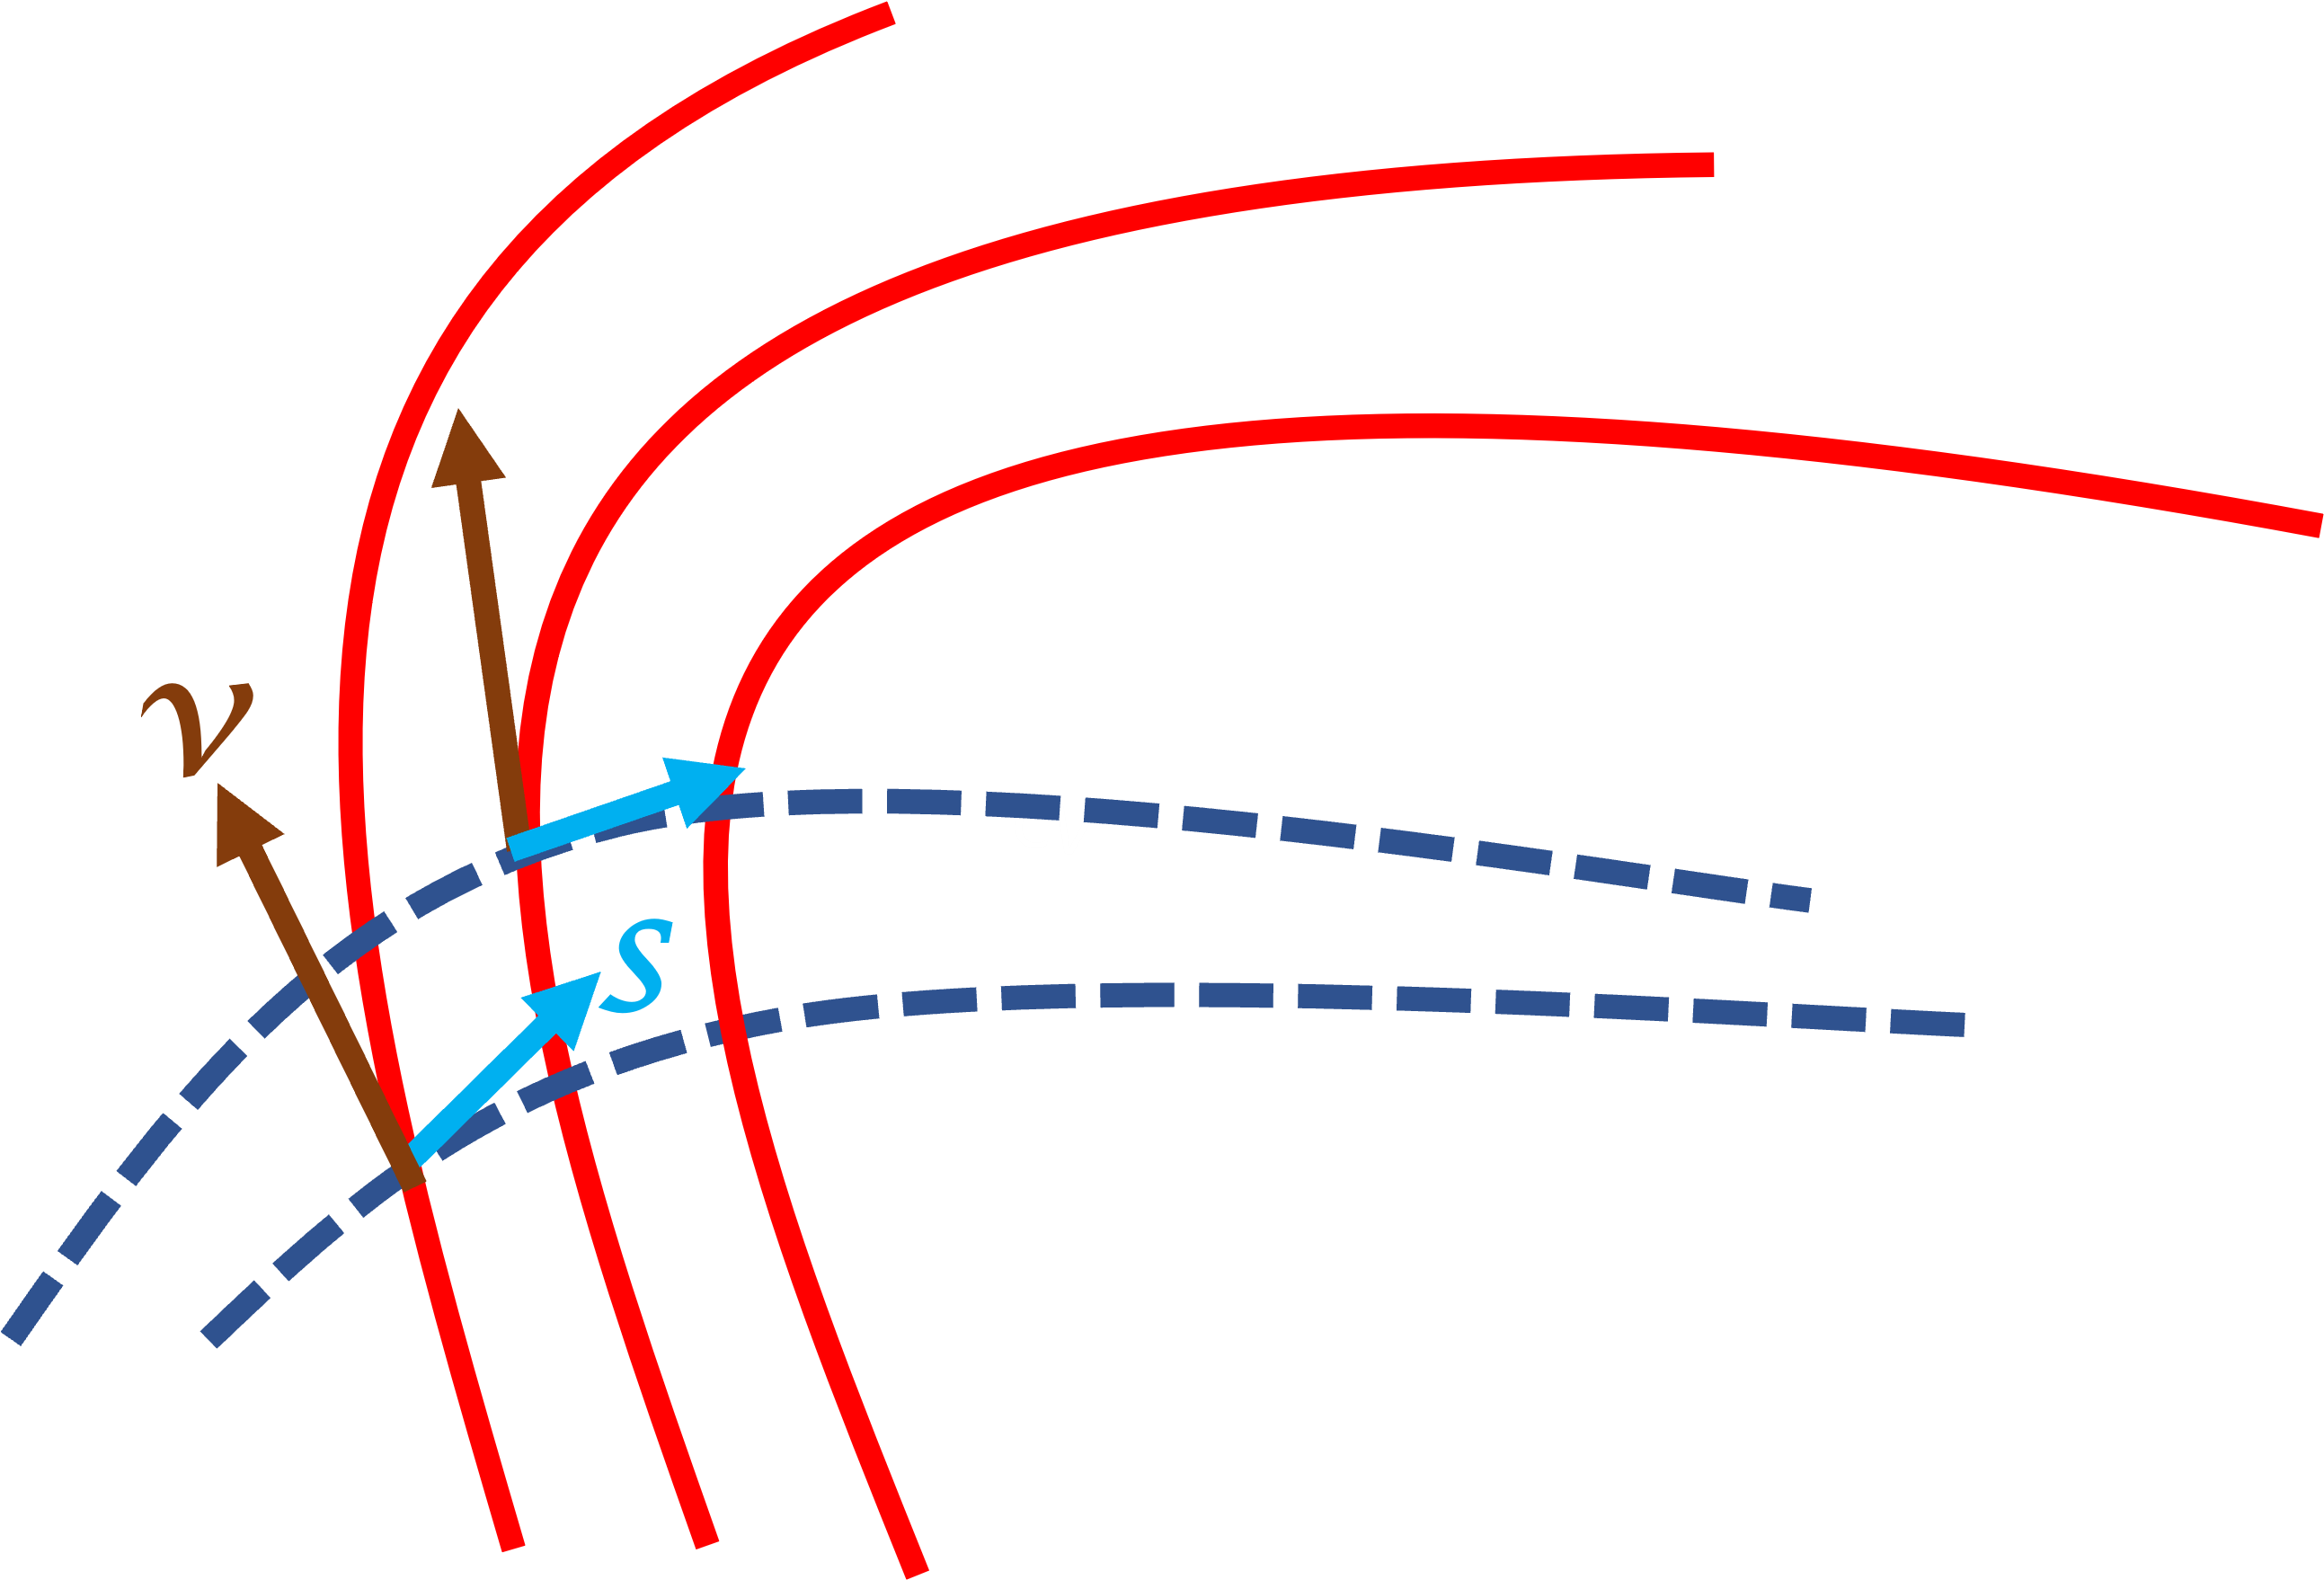
\includegraphics[width=0.8\linewidth]{img01.png}
     \caption{{Geodesics on some arbitrary surface. Note that $\mathbf{v}$ indicates the tangent vector to the geodesic $\mathbf{s}$ is the orthogonal vector that measures the distance between two geodesics.}}
     \label{fig:01}
   \end{minipage}
\end{figure}
\end{frame}
%
%
\begin{frame}
\frametitle{Getting into the Math behind Curvature}
We will start with some basic assumptions. Let $(M,g)$ be our Riemann Manifold.
\begin{itemize}
\item We choose $\nabla$ to be the connection whose torsion is $0$.
\item We will let the lie brackets of the vector fields $V$ and $S$ vanish.
\end{itemize}
\pause
Recall that in multi-variable calculus, we often used the second derivative to check curvature. This works because the second derivative measures the change of change of function. Change of function can occur even without curvature since the change can be uniform (linear). We will apply an analogous concept here by replacing the double derivative with double covariant derivative of the vector field $V$.
\pause
Note that the geodesic equation is given as the vector field whose parallel transport along itself is zero (i.e., covariant derivative with respect to itself is zero).
Thus, we have
\begin{align}
\nabla_{\vec{v}} \vec{v}=0
\end{align}
\end{frame}

\begin{frame}
\frametitle{Math behind Curvature}
Continuing,
\begin{align}
\nabla_{\vec{v}} \vec{v}=0
\end{align}
Taking covariant derivative with respect to $\vec{s}$ on both sides,
\begin{align}
\nabla_{\vec{s}}\nabla_{\vec{v}} \vec{v}&=0\\
\Rightarrow \nabla_{\vec{s}}\nabla_{\vec{v}} \vec{v}-\nabla_{\vec{v}}\nabla_{\vec{s}} \vec{v}+\nabla_{\vec{v}}\nabla_{\vec{s}} \vec{v}&=0
\end{align}
Using the definition of Riemann Curvature, the above equation reduces to
\begin{align}
\label{main_eq}
R(\vec{s},\vec{v})\vec{v}+\nabla_{\vec{v}}\nabla_{\vec{v}} \vec{s}=0
\end{align}
\end{frame}


\begin{frame}
\frametitle{More Figures}
\begin{figure}[!htb]
	\centering
   \begin{minipage}{0.3\textwidth}
     \centering
     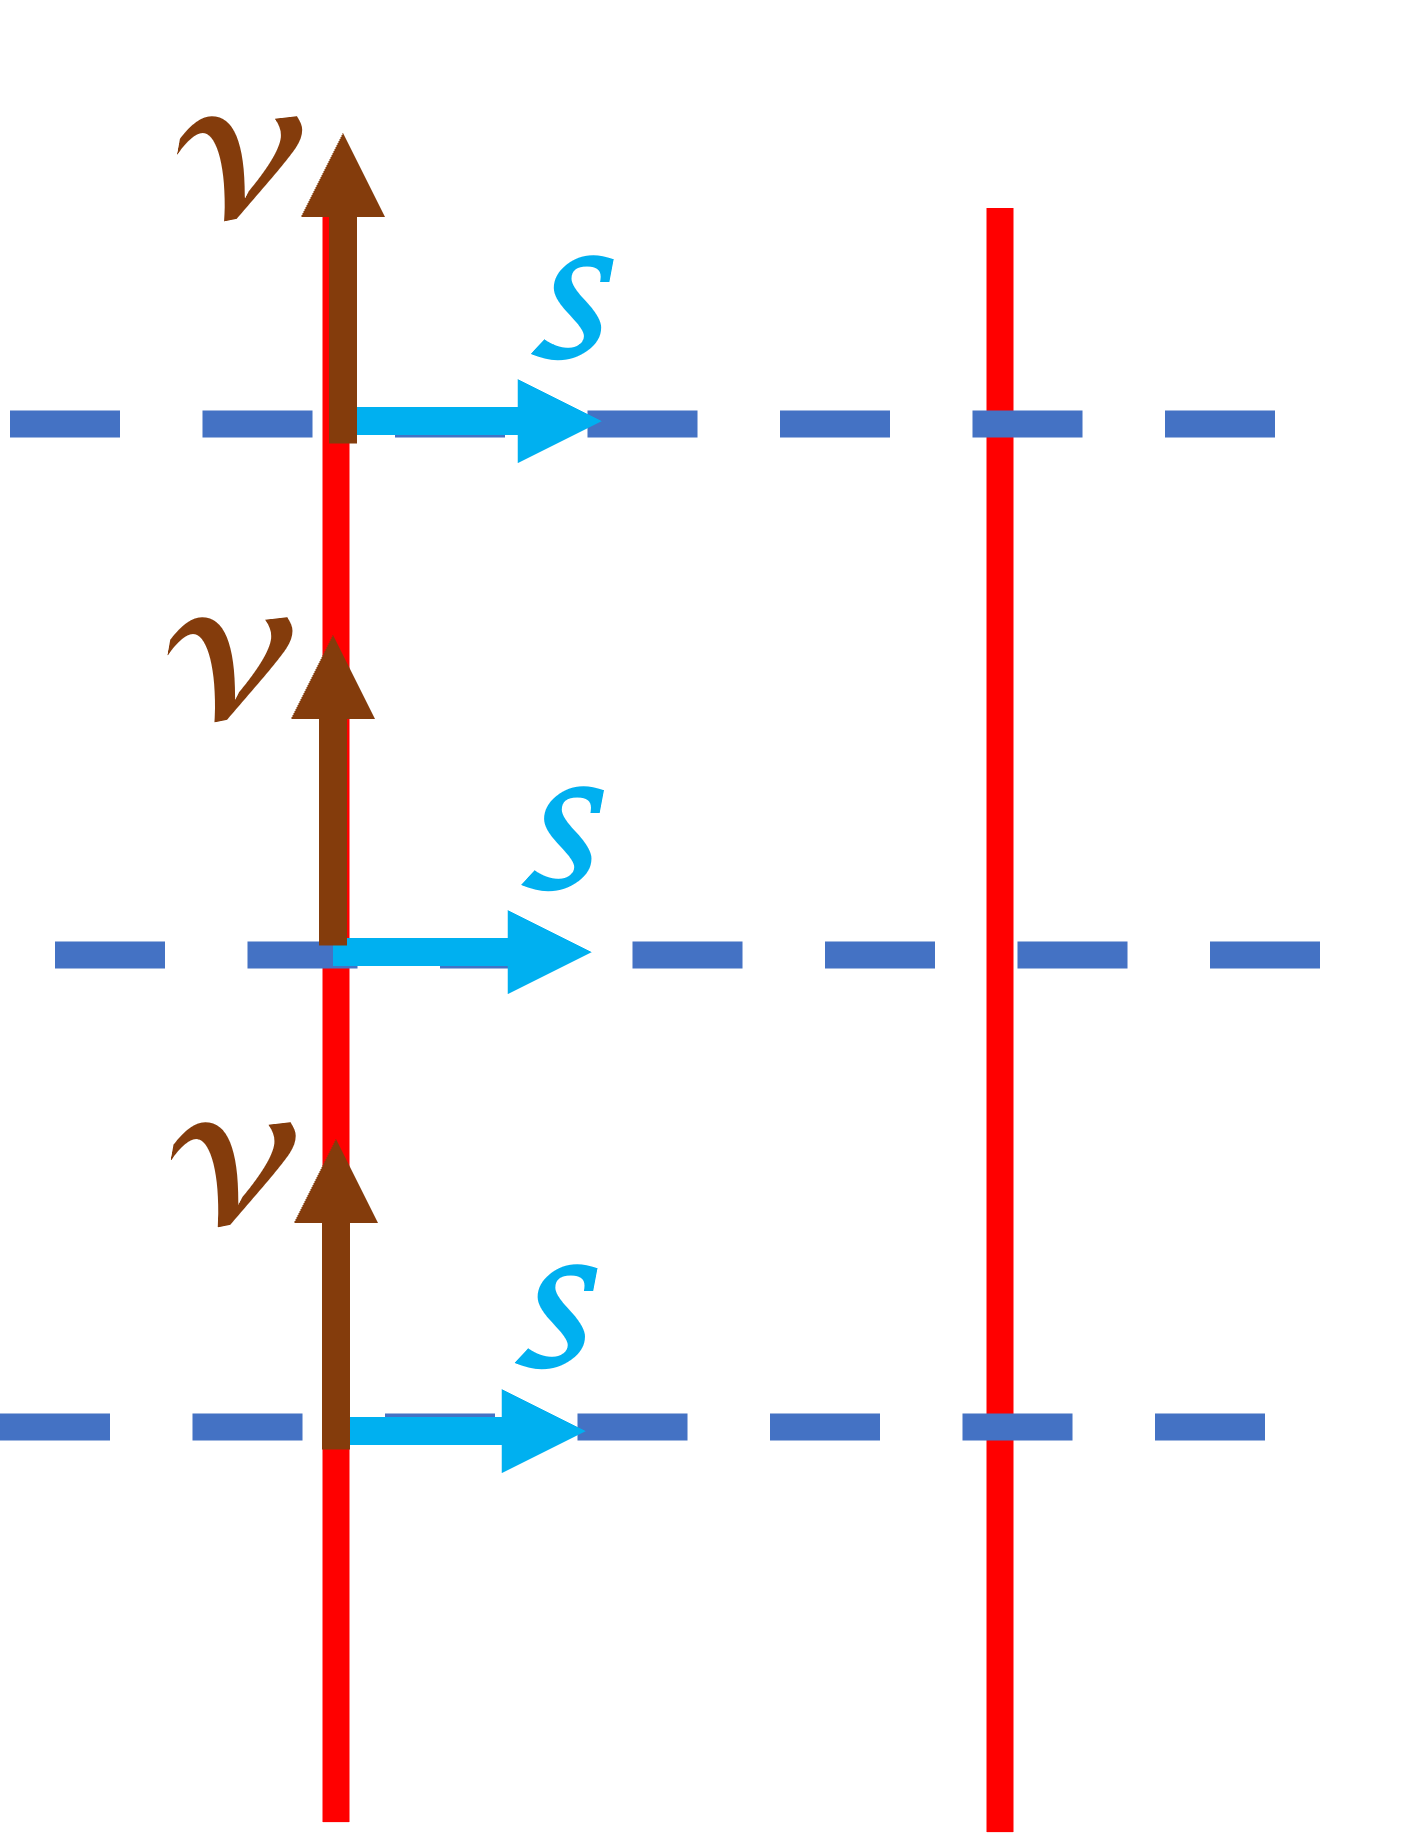
\includegraphics[width=\linewidth]{img02.png}
     \caption{{Case I: We have straight geodesics}}
     \label{fig:02}
   \end{minipage}
   \begin{minipage}{0.3\textwidth}
     \centering
     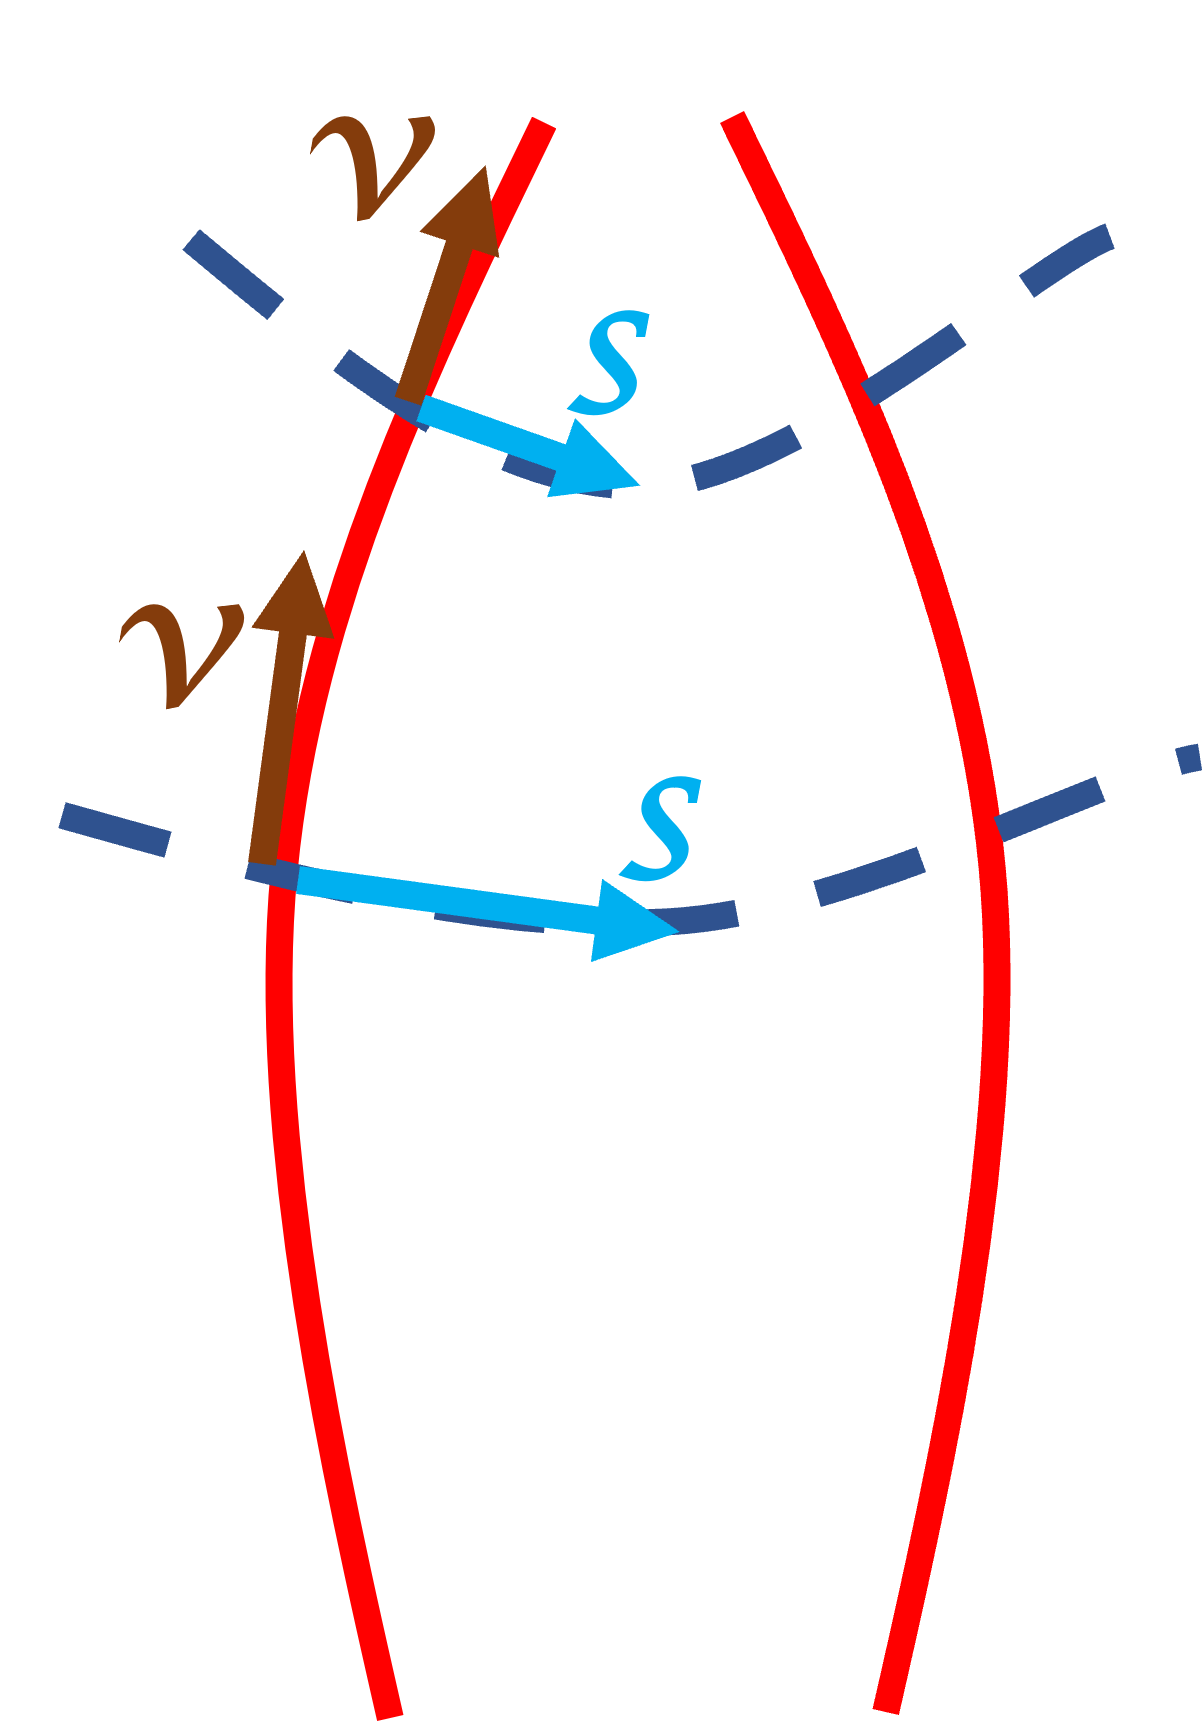
\includegraphics[width=\linewidth]{img03.png}
     \caption{{Case II: We have converging geodesics (positive curvature)}}
     \label{fig:03}
   \end{minipage}
   \begin{minipage}{0.3\textwidth}
     \centering
     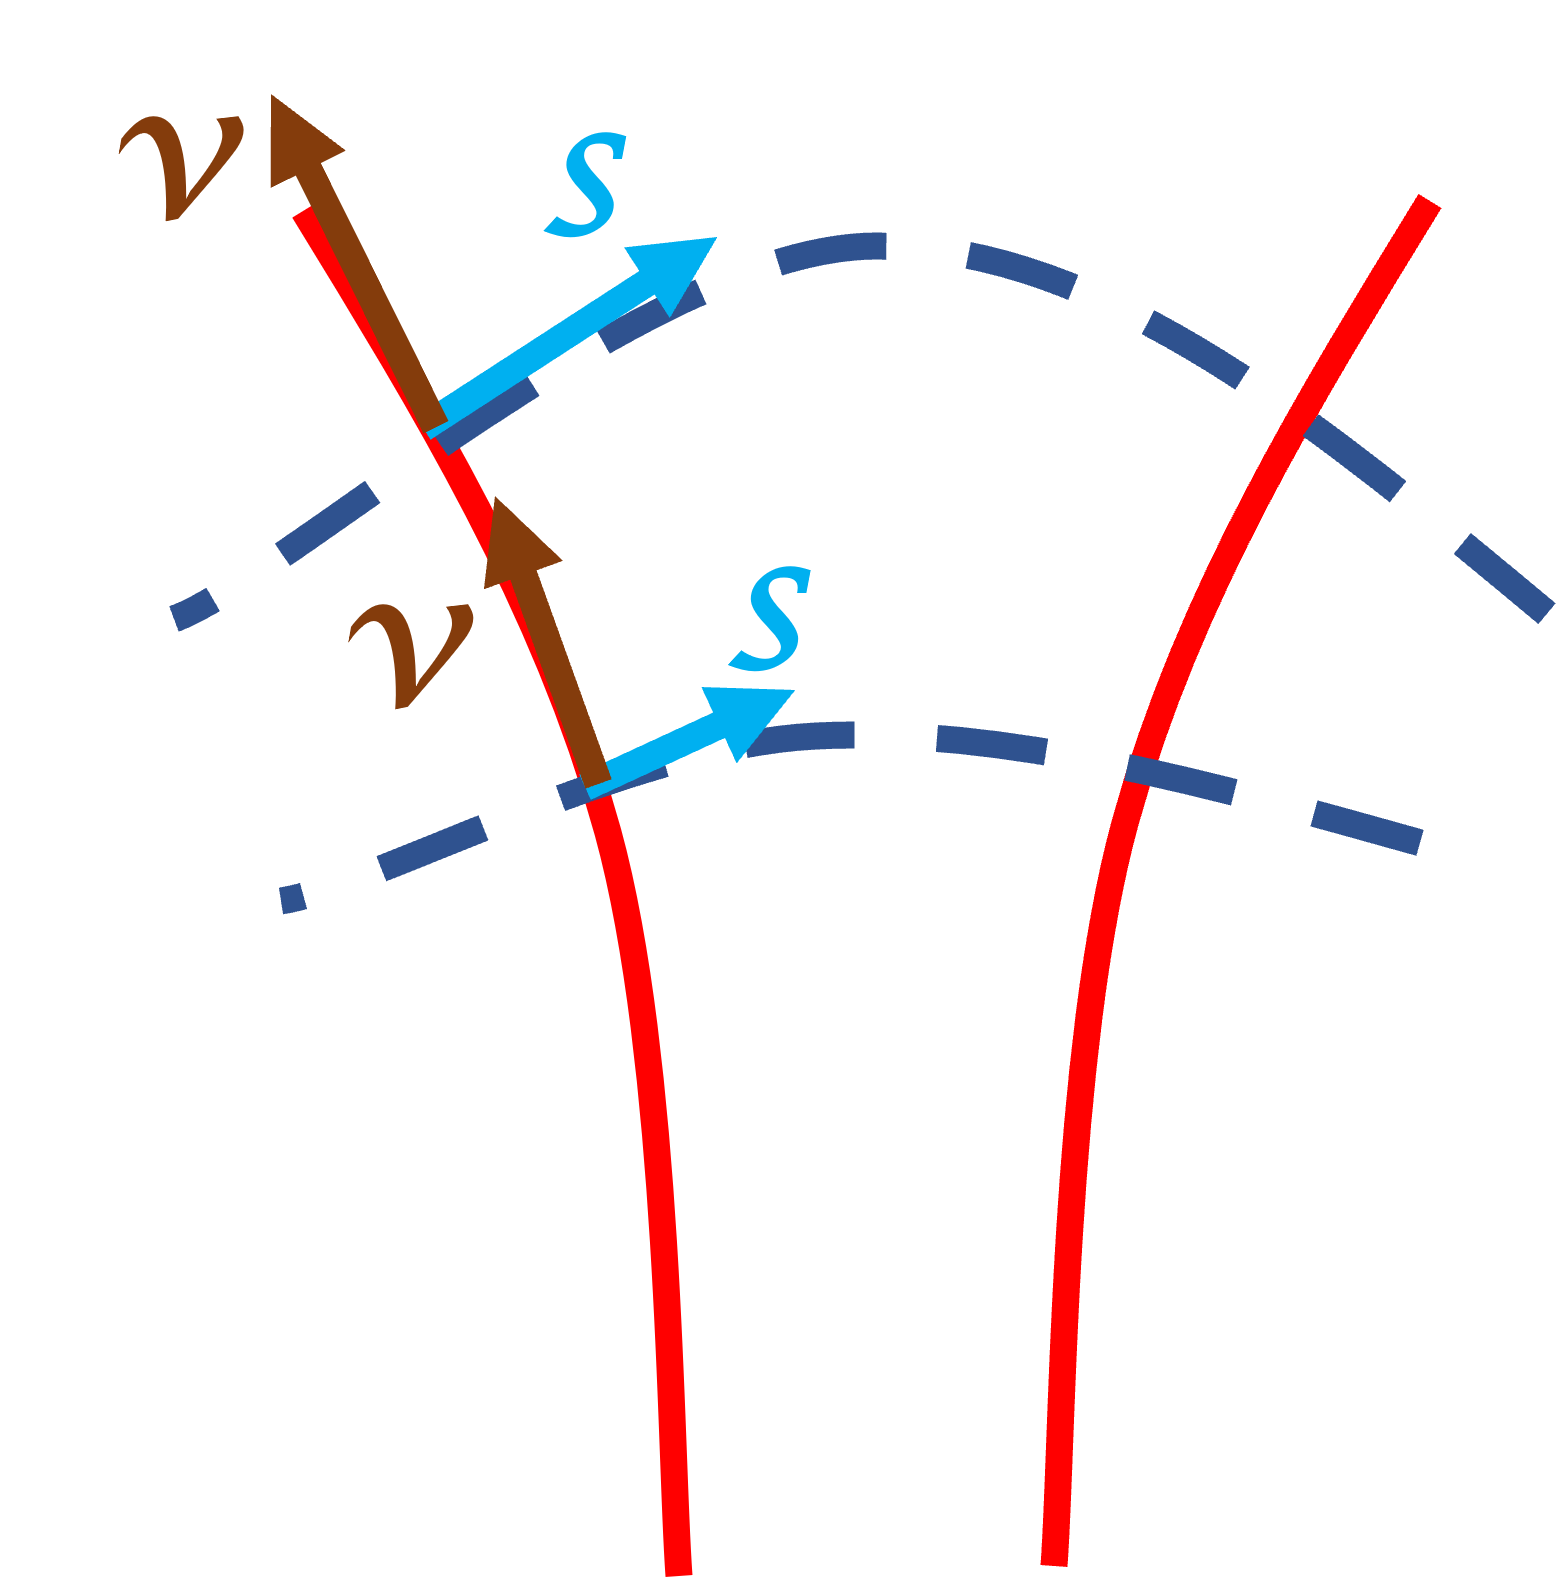
\includegraphics[width=\linewidth]{img04.png}
     \caption{{Case III: We have diverging geodesics (negative curvature)}}
     \label{fig:04}
   \end{minipage}
\end{figure}
\end{frame}

\begin{frame}
\frametitle{Figures Explained}
Note that $\nabla_{\vec{v}}\nabla_{\vec{v}} \vec{s}$ indicates the rate of change of how fast the $\vec{s}$ vector changes with respect to travelling on the geodesic. First we consider the sign. In case I, $\nabla_{\vec{v}}\nabla_{\vec{v}} \vec{s}=0$ (since $\vec{s}$ is uniform throughout the geodesic) . In case II, we have $\vec{s}$ decreasing in magnitude and this decrease decreases continuously. Thus, $\nabla_{\vec{v}}\nabla_{\vec{v}} \vec{s}=0$ is opposite to $\vec{s}$. This yields $\inner{\nabla_{\vec{v}}\nabla_{\vec{v}} \vec{s},\vec{s}}<0$. Using equation \ref{main_eq}, we get $\inner{R(\vec{s},\vec{v}) \vec{v}, \vec{s}}>0$. Likewise, for case III $\inner{R(\vec{s},\vec{v}) \vec{v}, \vec{s}}<0$. This is the intuition behind curvature.
\end{frame}

\begin{frame}
\frametitle{Is This It?}
We have intuitively concluded the form of curvature as $K(\vec{s},\vec{v})=\inner{R(\vec{s},\vec{v}) \vec{v}, \vec{s}}$, which holds true upto a constant. Note that curvature must be independent of the choice of basis. This can be done by suitable normalization.
\pause
Now onwards, we will drop the $\vec{.}$ symbol.\\
Consider a new set of basis $(\tilde{v},\tilde{w})=(av+bw,cv+dw)$ for $a,b,c,d\in\mathbb{R}$. The curvature should not change in this new basis. We will use the fact that 
\begin{align}
\norm{\tilde{v} \wedge \tilde{w}}&=\norm{av+bw \wedge cv+dw}\\
&=\abs{ad-bc}\norm{v \wedge w}
\end{align}
\end{frame}

\begin{frame}
\frametitle{Normalization: Part I}
Now,
\begin{align}
R(\tilde{v},\tilde{w})&=R(av+bw,cv+dw)\\
\label{tensor property 1}
&=R(av,cv)+R(av,dw)+R(bw,cv)+R(bw,dw)\\
\label{tensor property 2}
&=acR(v,v)+adR(v,w)+bcR(w,v)+bdR(w,w)\\
\label{anticommutative property}
&=(ad-bc)R(v,w)
\end{align}
where equations \ref{tensor property 1} and \ref{tensor property 2} use the multi linearity of tensors and equation \ref{anticommutative property} uses the fact that $R(v,w)=-R(w,v)$.
\end{frame}

\begin{frame}
\frametitle{Normalization: Part II}
Using $K(v,w)=\inner{R(v,w) w, v}$ from the previous slides, 
\begin{align}
K(\tilde{v},\tilde{w})&=\inner{R(\tilde{v},\tilde{w}) \tilde{w}, \tilde{v}}\\
\label{riemann property}
&=(ad-bc)\inner{R(v,w) \tilde{w}, \tilde{v}}\\
&=(ad-bc)\inner{R(v,w) av+bw, cv+dw}\\
\label{inner product property}
&=(ad-bc)^2\inner{R(v,w) v, w}
\end{align}
where equation \ref{riemann property} follows from equation \ref{anticommutative property} and equation \ref{inner product property} follows from the axioms of inner product of vectors.\\
\pause
Equation \ref{inner product property} shows that we need to scale down the curvature by $(ad-bc)^2$ in order to normalize it. 
\end{frame}

\begin{frame}
\frametitle{Final Result}
Thus, we can define curvature as
\begin{align}
\label{final result}
K(v,w)&=\frac{\inner{R(v,w) w, v}}{\norm{v\wedge w}^2}
\end{align}
We can show that the above quantity is indeed a tensor and invariant under a change of basis.
\end{frame}
\section{Problem 8 of Chapter 5 of Notes}
\begin{frame}
\frametitle{Problem 8 of Notes Chapter 5}
\begin{block}{Problem 8 of Notes Chapter 5}
Show that the sectional curvature of the sphere at all points is 1.
\end{block}
\end{frame}

\begin{frame}
\frametitle{Problem 8: Motivation}
We will derive the sectional curvature of a spherical surface of radius $R$. Note that while the calculations are straight-forward using the formulae for Christoffel symbols and Riemann tensor, the calculations are rather cumbersome and non-trivial. We aim to provide a detailed calculation of the various parameters, most of which may be skipped over due to want of time. The slides are however there to stay and will contain the detailed derivations.\\
\pause
Our basic layout is as follows:\\
\begin{figure}[!htb]
	\centering
   \begin{minipage}{0.8\textwidth}
     \centering
     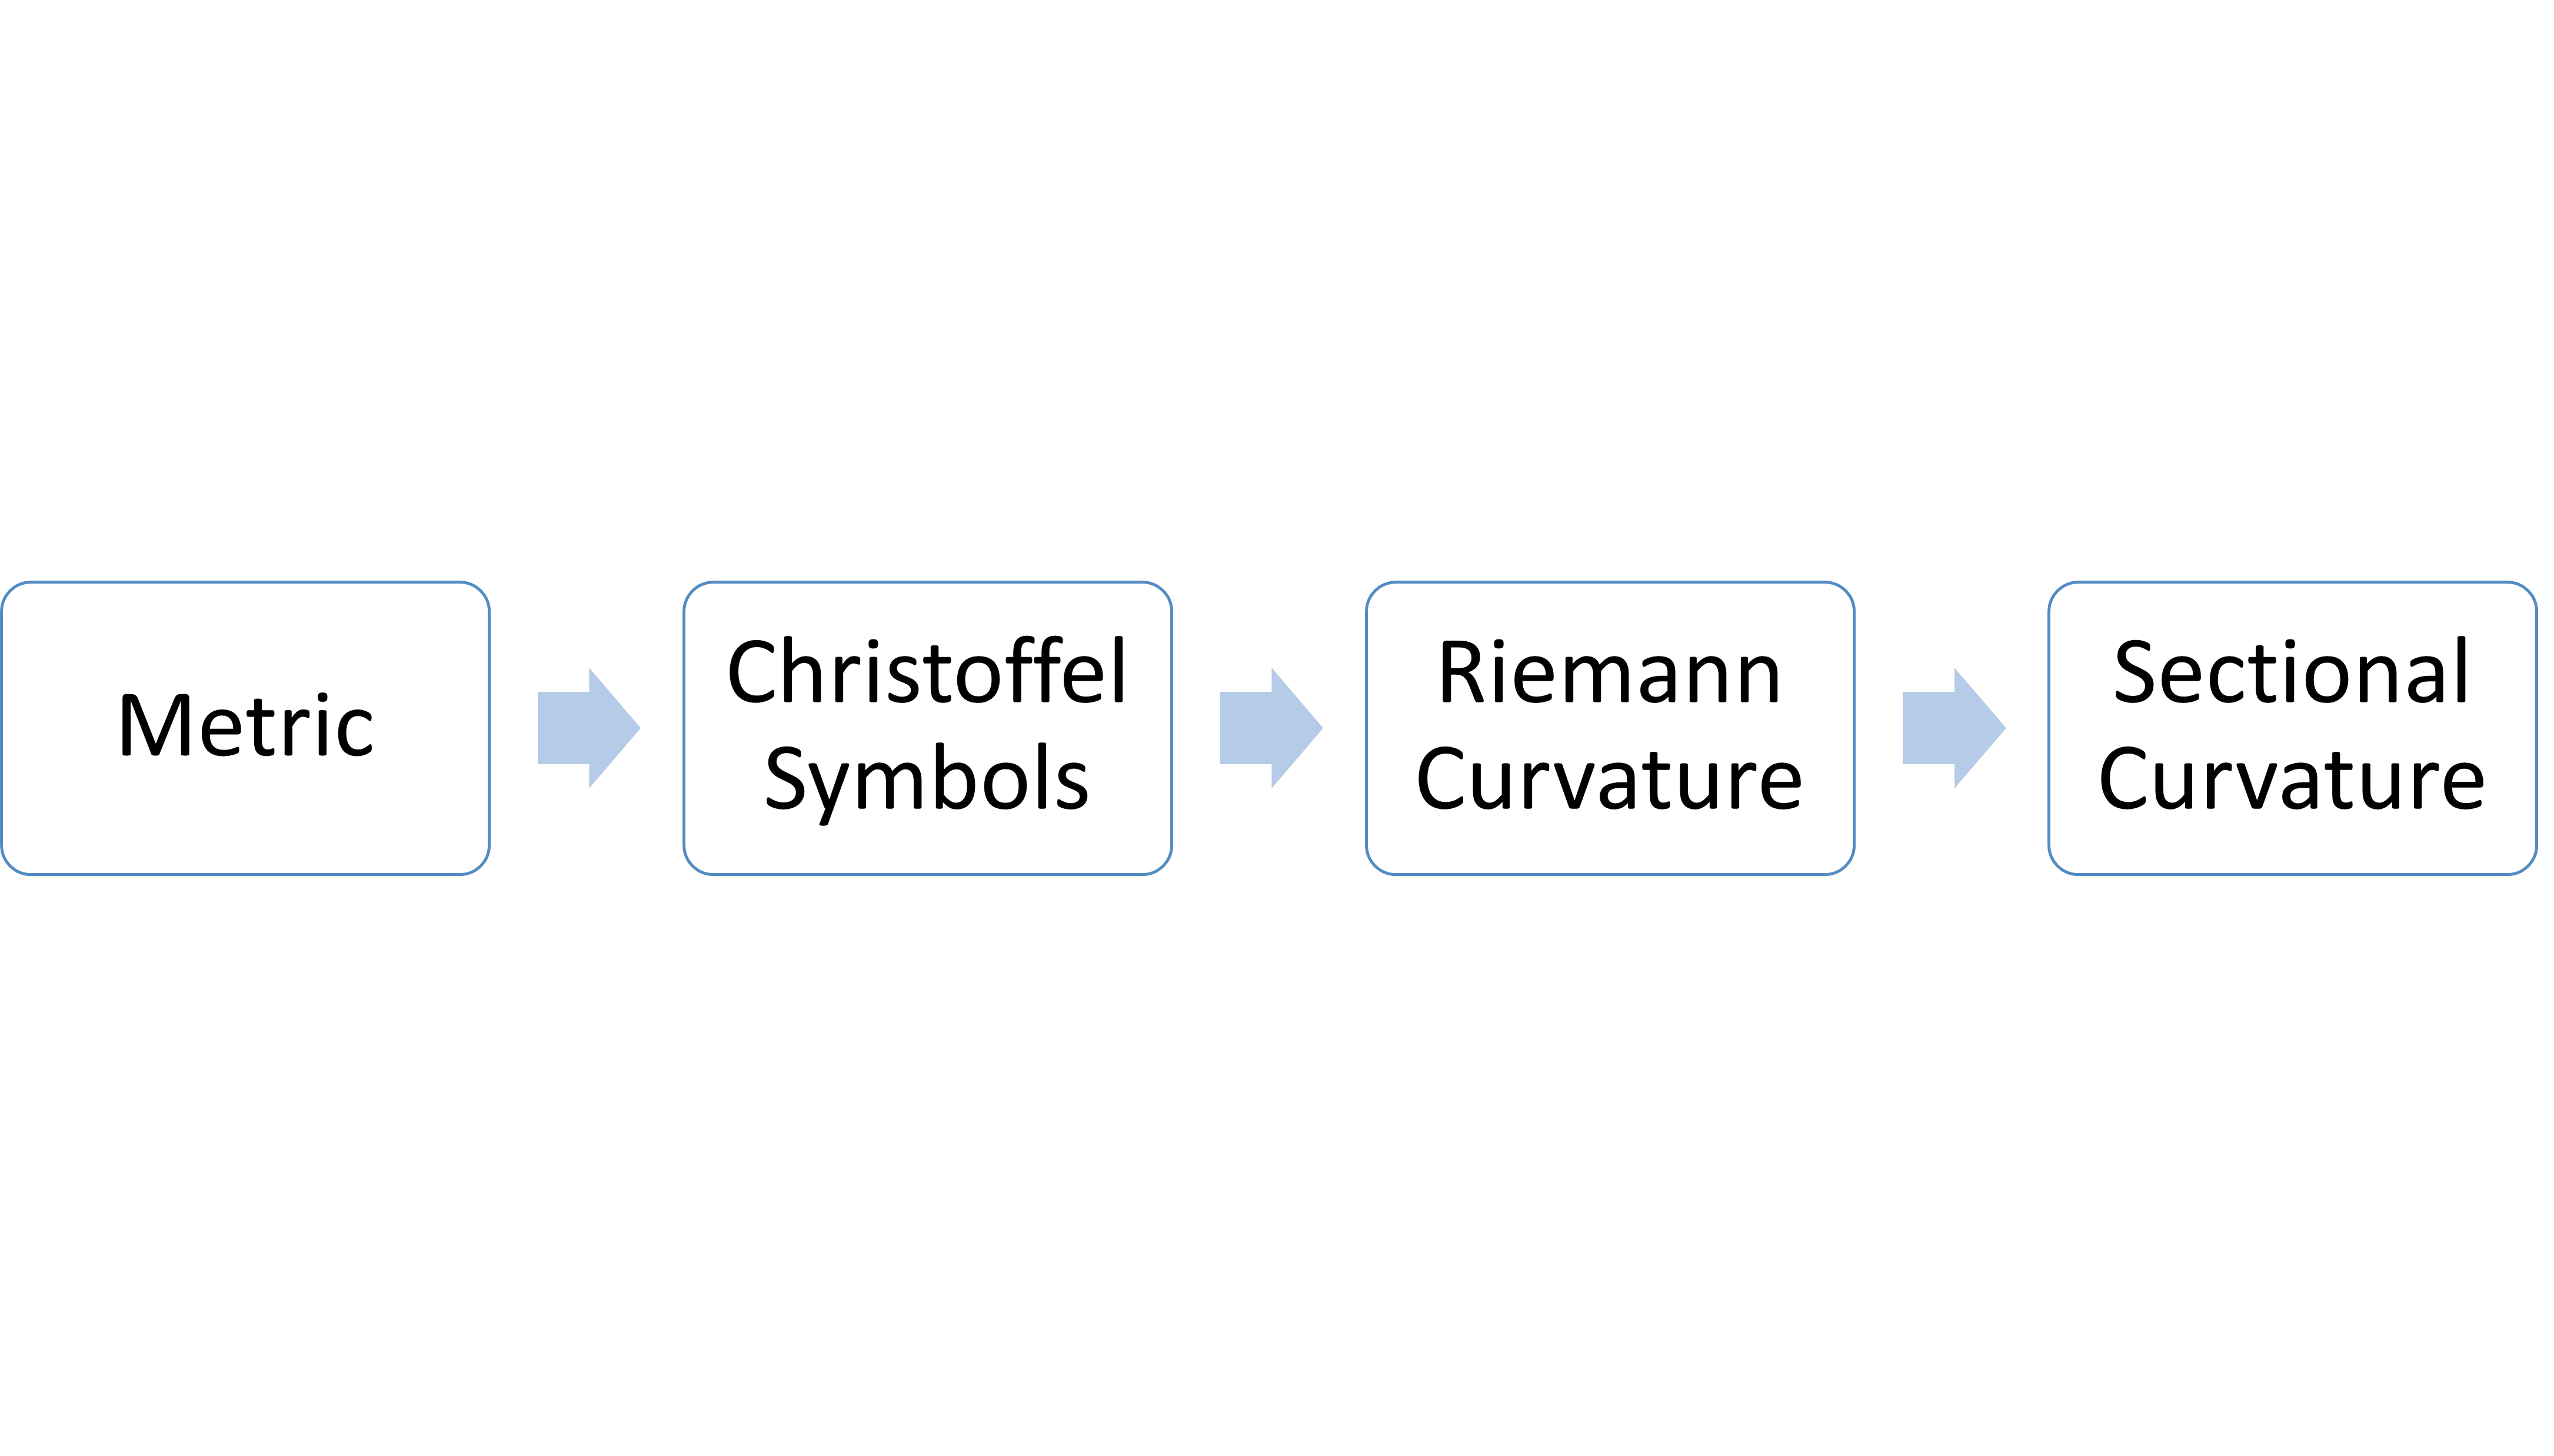
\includegraphics[width=0.5\linewidth]{img05.png}
     \caption{{Flowchart of our calculations}}
     \label{fig:05}
   \end{minipage}
\end{figure}
\end{frame}

\begin{frame}
\frametitle{Problem 8: Setting Up}
Some assumptions that we will make:
\begin{itemize}
\item We will assume the metric is given (this is one of the defining parameters of the manifold).\pause
\item We will follow the convention given in Do Carmo's book.\pause
\item We will use the formula for Christoffel symbols from metric.
\begin{align}
\label{christoffel symbols}
\Gamma^{\lambda}_{\mu\nu}=\bfrac{1}{2}g^{\lambda\alpha}(g_{\alpha\mu ,\nu}+g_{\alpha\nu ,\mu}-g_{\mu\nu ,\alpha})
\end{align}
where $\alpha$ is a dummy summation index.\pause
\item We will use the formula for Riemann curvature from Christoffel symbols (Lemma 5.5 of notes).
\begin{align}
\label{riemann curvature tensor}
R_{\lambda\mu\nu\sigma}=g_{\lambda\alpha}(\partial_\sigma\Gamma^{\alpha}_{\mu\nu}-\partial_\nu\Gamma^{\alpha}_{\mu\sigma}+\Gamma^{\alpha}_{\sigma\gamma}\Gamma^{\gamma}_{\mu\nu}-\Gamma^{\alpha}_{\nu\gamma}\Gamma^{\gamma}_{\mu\sigma})
\end{align}
where $\alpha$ and $\gamma$ are dummy summation indices.
\end{itemize}
\end{frame}

\begin{frame}
\frametitle{Problem 8: Specific Case of Sphere}
Note that out independent basis is formed by $(\theta,\phi)$ that span the surface of the sphere. The sphere is of radius $R$.\\ \pause
The distance metric is
\begin{align}
g=
\begin{pmatrix}
R^2 & 0\\
0 & R^2\sin^2\theta
\end{pmatrix}
\end{align}
i.e., $g_{\theta\theta}=R^2, g_{\theta\phi}=g_{\phi\theta}=0, g_{\phi\phi}=R^2\sin^2\theta$.\\ \pause
Calculating the inverse
\begin{align}
g^{-1}=
\begin{pmatrix}
\frac{1}{R^2} & 0\\
0 & \frac{1}{R^2\sin^2\theta}
\end{pmatrix}
\end{align}
i.e., $g^{\theta\theta}=\frac{1}{R^2}, g^{\theta\phi}=g^{\phi\theta}=0, g^{\phi\phi}=\frac{1}{R^2\sin^2\theta}$.\\
\end{frame}

\begin{frame}
\frametitle{Problem 8: Computing the Christoffel Symbols}
We will use equation \ref{christoffel symbols} to calculate the Christoffel symbols. We will also use the fact that the cross terms in the metric are zero.
\begin{align}
\Gamma^{\theta}_{\theta\theta}&=\bfrac{1}{2}g^{\theta\theta}(g_{\theta\theta ,\theta}+g_{\theta\theta ,\theta}-g_{\theta\theta ,\theta})=0\\
\Gamma^{\theta}_{\theta\phi}&=\bfrac{1}{2}g^{\theta\theta}(g_{\theta\theta ,\phi}+g_{\theta\phi ,\theta}-g_{\theta\phi ,\theta})=0\\
\Gamma^{\theta}_{\phi\theta}&=\bfrac{1}{2}g^{\theta\theta}(g_{\theta\phi ,\theta}+g_{\theta\theta ,\phi}-g_{\phi\theta ,\theta})=0\\
\Gamma^{\theta}_{\phi\phi}&=\bfrac{1}{2}g^{\theta\theta}(g_{\theta\phi ,\phi}+g_{\theta\phi ,\phi}-g_{\phi\phi ,\theta})=-\bfrac{1}{2}g^{\theta\theta}g_{\phi\phi ,\theta}=-\sin\theta\cos\theta
\end{align}
\end{frame}


\begin{frame}
\frametitle{Problem 8: Continuing the Computation of the Christoffel Symbols}
\begin{align}
\Gamma^{\phi}_{\theta\theta}&=\bfrac{1}{2}g^{\phi\phi}(g_{\phi\theta ,\theta}+g_{\theta\phi ,\theta}-g_{\theta\theta ,\phi})=0\\
\Gamma^{\phi}_{\theta\phi}&=\bfrac{1}{2}g^{\phi\phi}(g_{\theta\phi ,\phi}+g_{\phi\phi ,\theta}-g_{\theta\phi ,\phi})=\bfrac{1}{2}g^{\phi\phi}g_{\phi\phi ,\theta}=\bfrac{\cos\theta}{\sin\theta}\\
\Gamma^{\phi}_{\phi\theta}&=\bfrac{1}{2}g^{\phi\phi}(g_{\phi\phi ,\theta}+g_{\phi\theta ,\phi}-g_{\phi\theta ,\phi})=\bfrac{1}{2}g^{\phi\phi}g_{\phi\phi ,\theta}=\bfrac{\cos\theta}{\sin\theta}\\
\Gamma^{\phi}_{\phi\phi}&=\bfrac{1}{2}g^{\phi\phi}(g_{\phi\phi ,\phi}+g_{\phi\phi ,\phi}-g_{\phi\phi ,\phi})=0
\end{align}
\end{frame}

\begin{frame}
\frametitle{Problem 8: Riemann Curvature}
We shall calculate only $R_{\theta\phi\theta\phi}$ for calculating sectional curvature. It is straight-forwards but tedious to show that only the permutations of this tensor are non zero. We will use equation \ref{riemann curvature tensor}.
\begin{align}
R_{\theta\phi\theta\phi}&=g_{\theta\theta}(\partial_{\theta}\Gamma^{\theta}_{\phi\phi}-\partial_{\phi}\Gamma^{\theta}_{\phi\theta}+\Gamma^{\theta}_{\theta\theta}\Gamma^{\theta}_{\phi\phi}+\Gamma^{\theta}_{\theta\phi}\Gamma^{\phi}_{\phi\phi}-\Gamma^{\theta}_{\phi\theta}\Gamma^{\theta}_{\phi\theta}-\Gamma^{\theta}_{\phi\phi}\Gamma^{\phi}_{\phi\theta})\\
&=R^2(\sin^2\theta-\cos^2\theta-0+0+0-0-(-\sin\theta\cos\theta)(\bfrac{\cos\theta}{\sin\theta}))\\
&=R^2\sin^2\theta
\end{align}
\end{frame}

\begin{frame}
\frametitle{Problem 8: Sectional Curvature}
So far we have
\begin{align}
R_{\theta\phi\theta\phi}=R^2\sin^2\theta
\end{align}
Also, we have the formula for sectional curvature
\begin{align}
K(v,w)=\bfrac{\inner{R(v,w)w,v)}}{\abs{v\wedge w}^2}=\bfrac{R_{vwvw}}{\det(g)}
\end{align}
Hence, we get the sectional curvature of the sphere to be
\begin{align}
K(\theta,\phi)=\bfrac{R_{\theta\phi\theta\phi}}{\det(g)}=\bfrac{R^2\sin^2\theta}{R^4\sin^2\theta}=\bfrac{1}{R^2}
\end{align}
\end{frame}

\begin{frame}
\frametitle{Problem 8: QED}
Thus, for a unit sphere, curvature is constant ($=1$) at all points, irrespective of the values of $\theta$, $\phi$.\\ \pause
\begin{block}{Bonus}
What surface has constant negative curvature (say, -1)?
\end{block}

\end{frame}


\section{Riemann Curvature from Sectional Curvature}
\begin{frame}
\frametitle{Riemann Curvature from Sectional Curvature}
\begin{block}{Riemann Curvature from Sectional Curvature}
We can deduce the Riemann curvature at a point in the manifold given the sectional curvature of the surface.
\end{block}
\end{frame}


\begin{frame}
\frametitle{Motivation}
We will define some basic assumptions that we will use in out proof.
\begin{itemize}
\item Define 
\begin{align}
R(x,y,z,w)=\inner{R(x,y)z,w}
\end{align} 
\item Skew symmetry
\begin{align}
\label{skew	1}
R(x,y,z,w)&=-R(y,x,z,w)\\
\label{skew	2}
R(x,y,z,w)&=-R(x,y,w,z)
\end{align} 
\item Symmetry
\begin{align}
\label{sym}
R(x,y,z,w)=R(z,w,x,y)
\end{align}
\item Bianchi Identity
\begin{align}
\label{bianchi}
\sum_{\pi(x,y,z)}R(x,y,z,w)=0
\end{align}
\item Sectional Curvature
\begin{align}
K(v,w)=\bfrac{R(v,w,w,v)}{\norm{v\wedge w}^2}
\end{align}
\end{itemize}
\end{frame}

\begin{frame}
\frametitle{Setting Up}
Now, define a polynomial
\begin{align}
\label{polynomial f}
f(t)=&R(x+tw,y+tz,y+tz,x+tw)\\
&-t^2(R(x,z,z,x)+R(w,y,y,w))
\end{align}
Since all terms are symmetric, $f(t)$ can be expressed in terms of the sectional curvature and norm of wedge products. Thus, the RHS of equation \ref{polynomial f} is a polynomial in $t$ whose coefficients are the sectional curvatures.\\ \pause
Consider the coefficient of $t^2$ in equation \ref{polynomial f}. Using the multi linearity property of $R$ tensor, we can write it as
\begin{align}
f''(0)=R(x,y,z,w)+R(x,z,y,w)+R(w,z,y,x)+R(w,y,z,x)
\end{align}
\end{frame}

\begin{frame}
Using equations \ref{skew	1}, \ref{skew	2}, \ref{sym}, we obtain
\begin{align}
\label{coeff in f}
f''(0)=2R(x,y,z,w)-2R(z,x,y,w)
\end{align}
\frametitle{Some Simple Manipulations}
Now, exchange $x$ and $y$ and define a new polynomial
\begin{align}
\label{polynomial g}
g(t)=&R(y+tw,x+tz,x+tz,y+tw)\\
&-t^2(R(y,z,z,y)+R(w,x,x,w))
\end{align}
Since all terms are symmetric, $g(t)$ can again be expressed in terms of the sectional curvature and norm of wedge products. Following a similar procedure, we obtain
\begin{align}
\label{coeff in g}
g''(0)=-2R(x,y,z,w)+2R(y,z,x,w)
\end{align}
\pause
Now, \ref{coeff in f}-\ref{coeff in g} gives
\begin{align}
\label{riemann xyz}
f''(0)-g''(0)=4R(x,y,z,w)-2R(z,x,y,w)-2R(y,z,x,w)
\end{align}
\end{frame}

\begin{frame}
\frametitle{Completion of Proof}
Using \ref{bianchi},
\begin{align}
\label{substitution}
R(z,x,y,w)+R(y,z,x,w)=-R(x,y,z,w)
\end{align}
Substituting \ref{substitution} in \ref{riemann xyz},
\begin{align}
\label{final form}
f''(0)-g''(0)&=6R(x,y,z,w)\\
\Rightarrow &R(x,y,z,w)=\bfrac{f''(0)-g''(0)}{6}=\bfrac{(f-g)''(0)}{6}
\end{align}
\end{frame}

\begin{frame}
\frametitle{Final Result}
We need the polynomials $f$ and $g$ in terms of sectional curvature. Observe the form of $f$ in \ref{polynomial f}. Using the formula for sectional curvature,
\begin{align}
\label{f as sectional}
f(t)=&K(x+tw,y+tz)\norm{(x+tw)\wedge(y+tz)}^2\\
&-t^2(K(x,z)\norm{x\wedge z}^2+K(w,y)\norm{w\wedge y}^2)
\end{align}
Likewise
\begin{align}
\label{g as sectional}
g(t)=&K(y+tw,x+tz)\norm{(y+tw)\wedge(x+tz)}^2\\
&-t^2(K(y,z)\norm{y\wedge z}^2+K(w,x)\norm{w\wedge x}^2)
\end{align}
\end{frame}

\begin{frame}
\frametitle{Halloween Special: A Scary Expression}
Complete evaluation of equations \ref{final form}, \ref{f as sectional}, and \ref{g as sectional} gives an explicit formula for $R(x,y,z,w)$.
\pause
{\footnotesize
\begin{align*}
6\inner{R(x,y)z,w}=&K(x+w,y+z)\norm{(x+w)\wedge (y+z)}^2\\
&-K(y+w,x+z)\norm{(y+w)\wedge (x+z)}^2\\
&-K(x,y+z)\norm{x\wedge (y+z)}^2-K(y,x+w)\norm{y\wedge (x+w)}^2\\
&-K(z,x+w)\norm{z\wedge (x+w)}^2-K(w,y+z)\norm{w\wedge (y+z)}^2\\
&+K(x,y+w)\norm{x\wedge (y+w)}^2+K(y,z+w)\norm{y\wedge (z+w)}^2\\
&+K(z,y+w)\norm{z\wedge (y+w)}^2+K(w,x+z)\norm{w\wedge (x+z)}^2\\
&+K(x,z)\norm{x\wedge z}^2+K(y,w)\norm{y\wedge w}^2\\ 
&-K(x,w)\norm{x\wedge w}^2-K(y,z)\norm{y\wedge z}^2\\ 
\end{align*}
}%
Quite scary, isn't it?
\end{frame}





\begin{frame}
\begin{center}
THANK YOU!
\end{center}
\end{frame}

\begin{frame}
\frametitle{References}

\begin{enumerate}

\item
Notes, MA 556, Prof. Swapneel Mahajan, IIT Bombay, Autumn 2021

\item
Manfredo Perdigão do Carmo, \textit{Riemannian Geometry}, 2nd edition, 	Birkhäuser, 1992

\item
Jeff Cheeger and David G. Ebin, \textit{Comparison Theorems in Riemannian Geometry}, AMS Chelsea Publishing, vol. 365, 2008


\item
\url{https://www.maths.usyd.edu.au/PMH7/r/rg_emma_notes15.pdf}

\item
\url{https://www.youtube.com/watch?v=ZhDNijOEw0Y&ab_channel=eigenchris}


\end{enumerate}

\end{frame}

\end{document}